% !TeX spellcheck = en_GB
%\begin{wrapfigure}{r}{0.6\textwidth}
\begin{figure}
\centering
	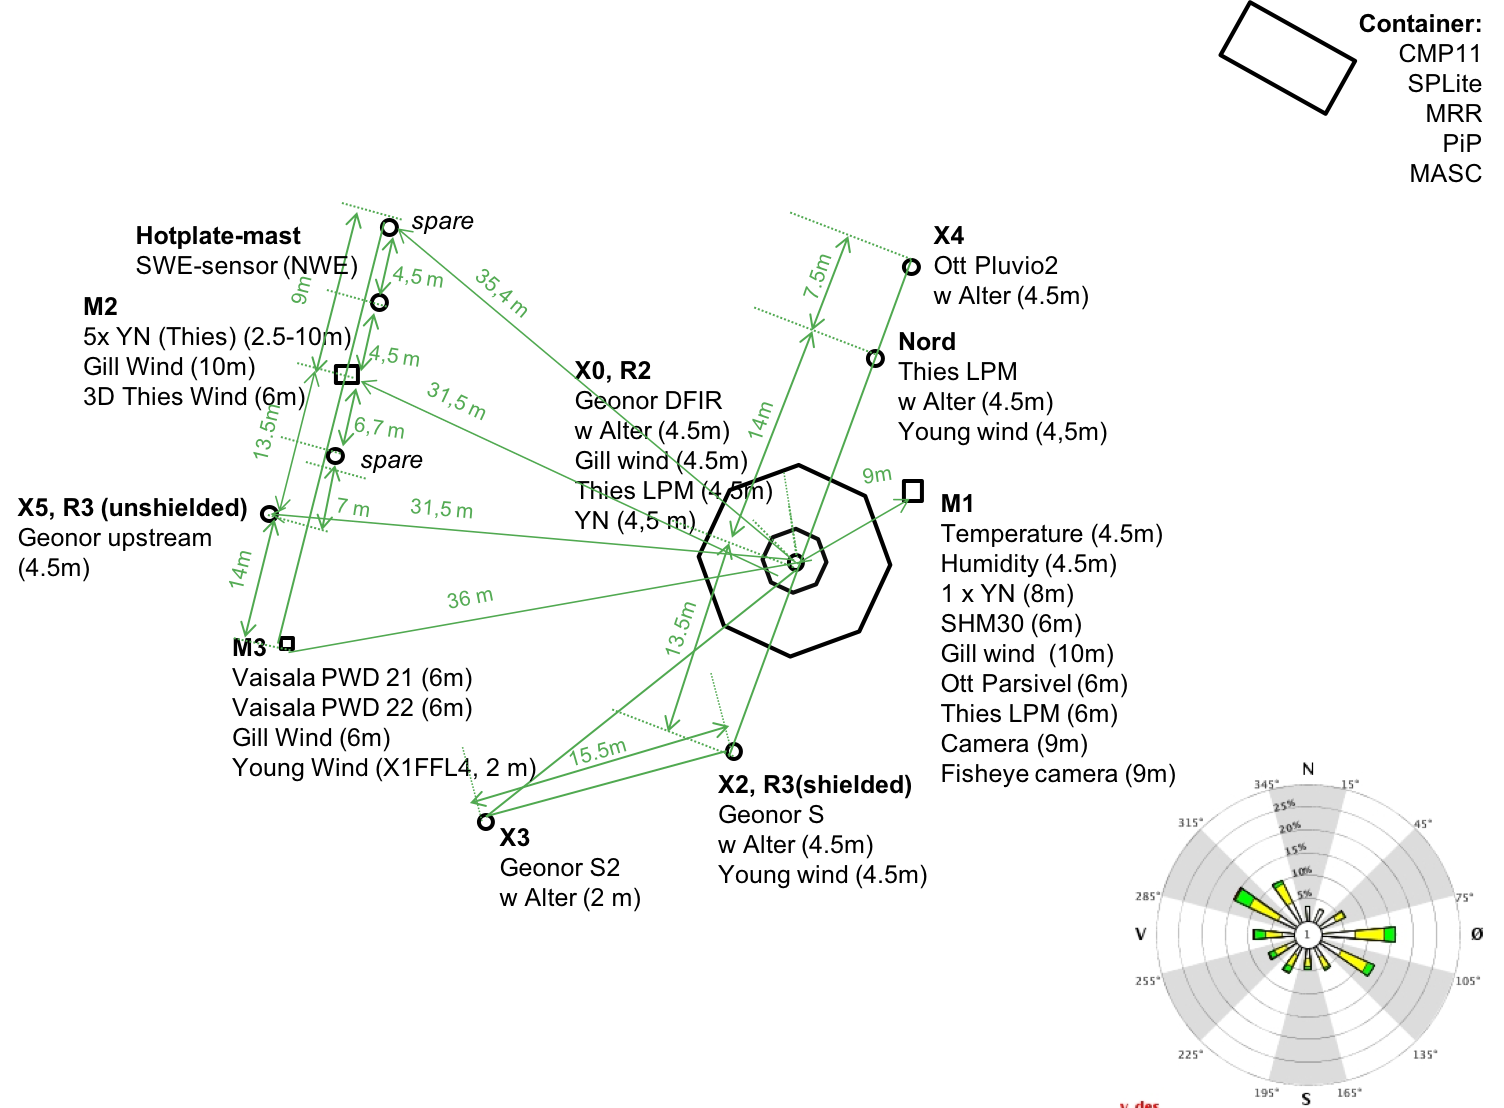
\includegraphics[width=\textwidth]{./fig_instruments/instrument_setting.png}
	%	\vspace{-10pt}
	\caption{Instruments at the Haukeliseter measurement site during winter 2016/2017 \citep[adapdet from][]{wolff_derivation_2015}. The windrose indicates the mean wind direction from either from west-north-west or east-south-east.}\label{fig:inst_setting}
\end{figure}
%	\vspace{-\normalbaselineskip}
	
%	\vspace{-\normalbaselineskip}
%\end{wrapfigure}